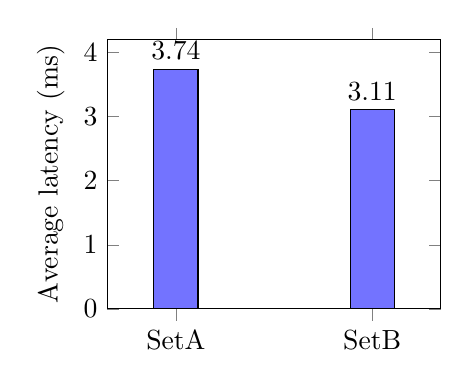
\begin{tikzpicture}
\begin{axis}[
  width=0.48\columnwidth,
  height=5.0cm,
  ybar,
  bar width=16pt,
  ymin=0,
  ymax=4.2,
  ylabel={Average latency (ms)},
  symbolic x coords={SetA,SetB},
  xtick=data,
  nodes near coords,
  enlarge x limits=0.35
]
\addplot[fill=blue!55] coordinates {(SetA,3.738) (SetB,3.106)};
\end{axis}
\end{tikzpicture}
\hfill
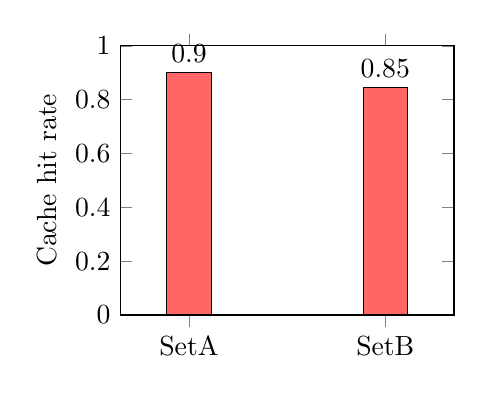
\begin{tikzpicture}
\begin{axis}[
  width=0.48\columnwidth,
  height=5.0cm,
  ybar,
  bar width=16pt,
  ymin=0,
  ymax=1.0,
  ylabel={Cache hit rate},
  symbolic x coords={SetA,SetB},
  xtick=data,
  nodes near coords,
  enlarge x limits=0.35
]
\addplot[fill=red!60] coordinates {(SetA,0.9) (SetB,0.8458333333333333)};
\end{axis}
\end{tikzpicture}
